
\section{Netzwerke}
Netzwerke setzen sich im allgmeinen aus $N$ Knoten (Nodes) zusammen, die über gewichtete Verbindungen (Edges) miteinander Verbunden sind. Besteht zwischen zwei Knoten eine Verbindung in beide Richtungen, so spricht man von einem ungerichteten Netzwerk. Wenn alle Knoten untereinander verbunden sind, so handelt es sich um ein vollständiges Netzwerk (siehe Abbildung \ref{fig:GraphBsp}).

\begin{figure}[t]
	 \centering
	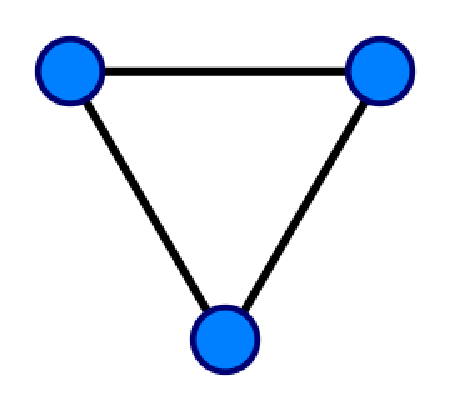
\includegraphics[width=0.3\textwidth]{abb/misc/GraphBsp.eps}
	\caption[Ungerichteres Netzwerk]{Beispiel eines ungerichteten Netzwerks aus drei Knoten, bei dem jeder Knoten mit jedem anderen Verbunden ist.}
	\label{fig:GraphBsp}
\end{figure}

\cite{pecora2014}
\cite{sagenotebook}
\cite{nauty}
\cite{pecora1998}